\documentclass[a4paper,12pt]{article}
\usepackage{times}
\usepackage[english]{babel}
\usepackage{durhampaper}
\usepackage{harvard}
\usepackage{graphicx}
\usepackage{fontspec}

\newfontface\lserif{Liberation Serif}

\newcommand{\Csh}{C{\lserif\#}}

\newcommand{\deliverable}[2]{\item \textbf{#1} --- #2}
\newcommand{\layer}[2]{\item \textbf{#1} --- #2\vspace{-1mm}}

\citationmode{abbr}
\bibliographystyle{agsm}

\title{AI for Autonomous Agents in Games and Simulations}
\author{James King}
\student{James King}
\supervisor{Magnus Bordewich}
\degree{BSc Computer Science}

\date{\today}

\begin{document}

\maketitle

\begin{abstract} {\bf Context:} Designing the core autonomous behaviour for characters in a video game, where those characters are expected by the player to perform tasks for themselves, poses many interesting challenges. This paper explores the tasks faced when developing a capable and somewhat convincing set of Artificial Intelligence routines within a simulated zombie epidemic as the foundation of a real-time strategy game with player allocated goals.
{\bf Aims:} The primary goal for this project was to develop a successful method of controlling a large number of agents in a hazardous environment to prioritise survival through cooperation. The algorithms must not be computationally expensive to allow for many agents to act in real-time and also express superficially convincing human-like behaviours.
{\bf Method:} Two conceptually distinct architectures for character behaviour were implemented, a subsumption stack and Beliefs-Desires-Intentions model. These were then compared in terms of the ability for agents to avoid threats, system resource usage and qualitative aspects of their behaviour. Advanced path finding and vision testing algorithms were also implemented.
{\bf Results:} A total of 480 individual simulations were performed to generate graphs describing population decline and execution speed for the subsumptive implementation and two versions of the BDI approach, which seemed to favour the BDI model for this scenario in all aspects.
{\bf Conclusions:} For this problem domain the BDI model appears to be a better fit due to its efficiency and power while also allowing for easy extensibility. A few avenues for additional research in the area of shared task planning are also identified.
\end{abstract}

\begin{keywords}
AI, BDI, cooperative, multi-agent, subsumption, task planning, video game
\end{keywords}

\section{Introduction}
\subsection{Context}\noindent
Video game worlds are often populated by computer controlled Non-Player Characters (or NPCS), the behaviour of which can make or break a game. A considerable amount of effort and care is required when designing the routines used by these characters if they are to satisfy the following major requirements. They should behave with approximate rationality, provide an appropriate challenge for the player and act in a believable way if the characters represent humans (or at least animals). For Real-Time Strategy (or RTS) games the difficulty is further accentuated by the necessity for the game to support perhaps hundreds or even thousands of these characters in an environment simultaneously. This combines the previous three requirements with a fourth: performance. Designing solutions for the first three key requirements is often more of a creative task than a purely methodical one and entails an element of subjectivity. The fourth requirement is easier to test, but the difficulty in maintaining a minimum performance quality heavily depends on the complexity of the solutions for the first three goals.

\subsection{Problem Domain}\noindent
This project aims to explore possible implementations of an NPC behaviour system designed to realise the central gameplay of a work-in-progress RTS game. The components of the game that existed prior to this project form a zombie epidemic simulation within a procedurally generated city environment containing buildings separated by streets constructed on a tile-based grid. Initially, a number of human characters are dispersed around the environment, a fraction of which are allocated the role of being a zombie. The simulation then begins, with the zombies navigating towards the nearest visible human and humans attempting to run away from danger if any is present (and otherwise just wandering randomly). If a zombie catches up to a human it may attack it, reducing a stored health value for that human and infecting that human with some probability. A human will become a zombie if they are infected when their health value reaches zero, while a zombie or non-infected human is simply removed from the simulation upon losing all their health.

The conflict is clearly one-sided, not least because the zombies are smarter than the humans. The humans have little regard for their surroundings other than the locations of visible enemies and so often run directly into the inner corners of walls. This would obviously not be classed as a sufficient behaviour as it does not meet the core requirements for a decent NPC. It fails at being rational, at providing an appropriate challenge (the humans don't stand a chance) and the agents certainly don't act like humans. Their only redeeming quality is that their simple AI isn't too computationally expensive, so thousands of them can be supported simultaneously.

\subsection{Project Aims}\noindent
At the very least the artificial intelligence routines explored in this project were expected to improve each human agent's survival ability. This may mean attempting to escape when cornered, deciding when it is rational to attack in self defence and implementing strategies to hide from danger. As an advanced objective this project would then explore implementing strategies for the human agents to autonomously construct barricades out of material found in buildings. This functionality would require an efficient path finding technique to be implemented, both for navigating away from danger and building barricades, but also to detect whether a region of the world is fully enclosed by barricades and therefore inaccessible.

The two core approaches to be compared are a Subsumption architecture \cite{brooks90} and a Belief-Desires-Intentions model \cite{rao95}, and the central research question for this project was to determine which of the two is most suitable for a real-time simulation involving many cooperating agents in a hazardous environment. A subsumption architecture features a stack of behaviour layers where each may in turn choose to either act or subsume control to the next layer, starting with the top of the stack. The first layer in the sequence to specify an action is heeded and the rest are ignored. This design usually relies on complex behaviour emerging from complimentary layers. A Belief-Desires-Intentions model is a radically different approach, where each agent records an internal representation of the world from which a set of attainable goals are found, a subset of which are committed to in an attempt to maximise expected utility.

\subsection{Deliverables}\noindent
These following core elements were created for this project.

\begin{enumerate}
  \deliverable{Expanded Core Game}
  {The main environmental components that the AI system utilises were implemented. These include the creation of game objects that represent a resource to be used when building barricades, the system to support the construction of the barricades themselves, the implementation of an efficient path finding system, and utilities to allow for visibility and collision testing.}

  \deliverable{Subsumption Prototype}
  {An agent design using a subsumption architecture was developed, implementing the core requirements of the human NPCs. This prototype was constructed by breaking up the humans' functionality into a stack of behaviours, from which a successful strategy was designed to emerge.}

  \deliverable{BDI Prototype}
  {A distinct agent design using a BDI architecture was also developed, meeting the same requirements as the subsumption approach. This prototype involved personal abstracted representations of the environment for each human agent, from which a set of achievable goals are found using a goal evaluation algorithm. These goals are then further reduced into a set that is calculated to yield the most utility and are simultaneously possible.}

  \deliverable{Analysis \& Comparison}
  {Both completed prototypes were analysed and compared in terms of agent survival rate, prevalence of unnatural behaviour and system resource usage. The bulk of this analysis involved a set of graphs describing the change in agent population over time and simulation performance from a wide variety of situations, from which it was determined that the BDI approach outperformed the subsumptive ones in many respects. Possible extensions to the algorithm were also identified, which may be an avenue for additional research.}
\end{enumerate}

\section{Related Work}
Before construction of the two AI prototypes could begin, an efficient shortest-path finding algorithm needed to be found. Solving this problem can be costly when applied to complex environments or when using many agents if an approximately optimal result is desired. The goal is to emulate the human ability to plan a route through a world (or an abstraction of one), usually with complete knowledge of the environment to be navigated. It is far more difficult to find an optimal path if aspects of the world are hidden from an agent while it is planning a path, so a trade-off can be made to only require a path that is \emph{rational}. For games, a laxer requirement for the quality of path may even be beneficial, as the resulting path-finding agents appear more natural and human like, making occasional wrong turns along the way.

Computer games are real-time applications; they should respond to the actions of the player within a few milliseconds. The minimum requirement is to simulate and update the world between each consecutive pair of frames rendered and outputted to the screen. Conventional path finding algorithms such as A* \cite{hart68} will produce a complete and optimal path from the agent's position to the target position, a result that is quite costly and often unnecessary. \citeasnoun{bulitko10} describes and compares several algorithms that are designed to have a low time and memory footprint, and so are ideal for use in video games. The three algorithms analysed in detail are k Nearest Neighbours Learning Real-time A* (kNN LRTA*), Time-Bounded A* (TBA*), and Real-time Iterative-deepening Best-first Search (RIBS).

The first algorithm, kNN LRTA*, relies on a precomputed database of paths between \emph{subgoals}. This allows the bulk of path calculation to be offset to when the game world is created, and the time needed to find a path for each agent is significantly reduced. A decent heuristic for deciding which nodes to precompute paths between would be \emph{bottlenecks} in the game world, nodes that are more likely to be on paths between disparate regions of the world. For the on-line searching procedure, the main challenge is selecting a series of subgoals that would lead to the least deviation from the shortest path. In terms of optimality, the algorithm will trivially produce an optimal result if the starting and goal nodes are both subgoals with precomputed paths (assuming the precomputed paths are optimal - which they may well be depending on the algorithm used to find them). The article's performance analysis of the algorithm demonstrates the mean move time and sub-optimality of the algorithm as the size of the precomputed database increases. As would be expected, a larger database produces significantly more optimal results, although it appears to plateau at around 12 percent longer than optimal. A sub-optimality of this order is certainly sufficient for use in this project. The algorithm compares very favourably in both respects to the second algorithm, TBA*, and also in working memory used, but at a cost; a significant pre-computation time is required, in the order of several days for database sizes that produce even acceptable results. This could be a major issue if the algorithm were to be used for this project, because game worlds should be generated and therefore paths precomputed whenever a player wishes to begin a new game. Usually this doesn't pose a problem for games with static worlds, as the subgoal database may be precomputed by the developer and the results distributed with the game. The problem may be less pronounced when applied to this project as the pathing node count will be significantly smaller than the worlds used in their study, but the precomputation time would still add an unwelcome delay to the already lengthy world generation process.

The next algorithm analysed in the article is TBA*, a simple modification of the ubiquitous A* algorithm that simply limits the execution time to a fixed threshold. If the algorithm hasn't halted when the threshold is exceeded (a complete path has not been found), the immediate action that appears most promising is chosen. Another slight alteration is that the working data used by A* isn't discarded when an action is taken, and persists to the next simulation iteration to allow the agent to continue where it left off. For applications where there is adequate time to complete a full A* search every simulation step, this algorithm is clearly optimal. The time bounded nature of the algorithm essentially enforces a contract that the algorithm has constant worst-case time complexity, and so is suitable for real-time applications. However, the algorithm can occasionally reconsider which path to take and will produce movements that appear indecisive. This algorithm would certainly seem adequate for this project, and would inspire some aspects of the final path-finding implementation used.

Finally, the article describes the RIBS algorithm. This method attempts to be more agent-oriented than the previous algorithm in that TBA* will often explore nodes at locations in the map away from the agent it seeks to find a path for. In contrast, RIBS will focus on the agent's local environment and so will be able to respond to nearby changes and will involve less random access of remote nodes; beneficial in the case of expensive memory access. This algorithm is much more involved than TBA*, and may only provide limited improvements in efficiency. The technique is also relatively untested and so may have unforeseen drawbacks.

The second article to be analysed is \citeasnoun{buro05}, and details the Partial Refinement A* (PRA*) algorithm. This is another real-time path planning algorithm that relies on a tiered structure of the environment at different abstraction levels, and a heuristic function that can estimate the distance between two nodes at any abstraction level. The range of levels in this hierarchy spans from the original graph of path nodes in the world at the lowest level, to an unconnected graph with a node for each island of nodes from previous tiers with existing paths between them. Each tier is constructed such that within each abstracted node is a clique of nodes from the previous tier (although orphans are additionally attached to the group they connect to). A useful consequence of the construction of this hierarchy is the efficient ability to test if a path exists between any two nodes; simply check if they both belong to the same highest-level abstracted group. This can save a great deal of time because searching for a non-existent path can lead to a fruitless search through every node in the world. PRA* expands upon a simpler algorithm \emph{QuickPath}, which recursively finds and refines paths through each abstraction level from the highest to lowest, arriving at a complete path from the start to the goal node at the lowest abstraction level.

The article points out that while \emph{QuickPath} is guaranteed to find a path if it exists, there is little effort made to refine the path in an optimal manner and the result may be far longer than the shortest. The PRA* algorithm aims to improve the quality of the outputted path through several means. Firstly, the algorithm starts at a lower abstraction tier than the top layer, using A* to find a path of abstracted nodes. This abstracted path may then be refined recursively with subsequent A* calls. The method can be applied in an agent-centric way like RIBS, by only refining the path to the lowest abstraction near to the agent, saving computation time and allowing for a dynamic environment. This partial refinement can be compared to TBA* and RIBS from the previous article in that these algorithms don't attempt to produce a complete path from the agent to its destination, and simply do the best they can with the time they are allocated. However, PRA* should be less inclined to stumble into dead-ends than TBA*. The algorithm also suits this particular application well, as the world is already abstracted into groups of nodes in the form of the blocks containing each building; an abstracted path may be found at the block abstraction level and then partially refined for each block when it is visited by the path finding agent. Due to these merits the PRA* algorithm was chosen for this project, although with a path-finding request queueing system that is processed within allocated time periods in a similar manner to TBA*.

The first prototype required the implementation of a subsumption architecture, which is characterised by an ordered stack of layers that each implement an atomic behaviour for an agent \cite{brooks90}. The top-most layer decides whether to act or delegate control to the second layer, which in turn may delegate control to the third layer, and so on down the stack. The ordering of the layers should therefore represent the priority of their respective behaviours, with critical actions like threat avoidance at the top. The architecture was developed by \citename{brooks90} with the intention of prioritising an understanding of the interactions between the agent and its environment over prior approaches that focus on the manipulation of abstract symbols, as described in \citeasnoun{brooks90}. He argues that breaking concepts about the environment into individual symbols with defined relations and then expecting intelligence to emerge through the manipulation of those symbols would involve an unworkably large search space. His alternative is to avoid trying to internally model an abstraction of the environment through symbolic language, and instead simply use live observations from the world itself. His subsumption architecture is therefore designed around this notion of tightly binding an agent's behaviour with environmental perception.

While initial designs of the architecture used augmented Finite State Machines \cite{brooks86} due to limited computational resources at the time, today we have far more powerful devices at our disposal and so can use more developer-friendly programming paradigms. An example of a modern implementation of the subsumption architecture is provided in \citeasnoun{butler01}. Their design is heavily object-oriented, with the subsumption stack being comprised of many BehaviourLayer objects that individually implement different behaviours. These objects receive the environment state through a \emph{doFeedback()} method, and then act by returning a set of actions from a \emph{doGo()} method which may block the invocation of lower layers. A very similar approach is used for the implementation in this project, with the exception of the two methods being merged into one that simultaneously observes and acts.

For the second prototype a BDI implementation was required, which is described in \citeasnoun{rao95} as involving each agent maintaining an internal database of beliefs about the environment that is used to produce a set of desires based on an agent's goals. These desires are then filtered, with the remaining ones committed to for a period of time as intentions. The implementation in this project follows a similar main-loop structure as is specified by \citename{rao95}. First the agent generates a set of options that individually work towards separate goals based on the current beliefs model state. These are then compared and reduced down to a selected set that are expected to be non-conflicting. From this set intentions are either updated or replaced depending on whether the options align with any existing intentions, and then actions are performed as dictated by those intentions. Finally, the outcome of those actions are used to decide whether any intentions have been completed or are now impossible, and in either case those respective intentions are dropped.

\section{Solution}
\subsubsection{Development Environment}\noindent
This project is built on top of a game written in \Csh, targeting the .NET Framework version 4.5. Microsoft's Visual Studio 2013 was used as the integrated development environment for its \Csh~compiler, debugging and profiling tools and Sublime Text 2 for any peripheral text editing. Most of the development and all evaluation was performed on a Windows desktop PC (Intel Core i5, AMD 7850), using a Windows laptop (Intel Core i7, nVidia GeForce GT 540M) to test compatibility with nVidia GPUs. The OpenTK library is used to expose OpenGL bindings for .NET and is the only non-standard library used.

\subsubsection{High Level Architecture}\noindent
After the environment has been generated a main control loop begins. During each iteration this loop will either perform a simulation step, redraw the screen, or both; depending on how much time has passed since those respective actions were last performed. While screen redrawing will occur as frequently as possible while maintaining a minimum period of 16.67ms, simulation steps attempt to maintain an average period of that same frame-time. This may involve running slightly more simulation steps than the desired average to make up for a prior period of slow updates that fell below the average. Each simulation step cycles through every object in the game environment, including agents, and allows them to perform some individual logic. Following this, any player inputs are interpreted and the path finding queue is processed as described in section \ref{sec:paths}.

\subsubsection{Path Finding \& Navigation}\noindent
The problem of finding efficient paths through virtual environments is often faced when developing AI for games and so has been explored extensively. Generally the A* algorithm \cite{hart68} is used, although while it guarantees a high quality path it may require a significant amount of time to find it (depending on the complexity of the environment). When observing the structure of the worlds produced by the procedural city generation algorithm (See Figure~\ref{fig:block}) it is easy to spot aspects that can be exploited to produce an A* adaptation which is expected to require less time to execute.

\label{sec:paths}
\begin{figure}[h]
\centering
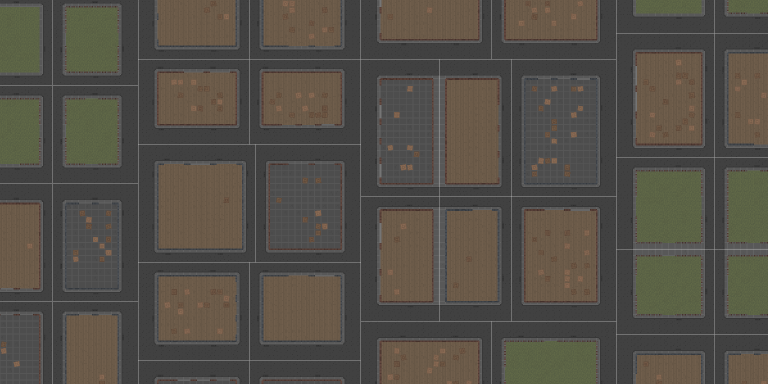
\includegraphics[width=0.9\textwidth]{blocks}
\caption{A diagram to show the structure of a procedurally generated city environment, featuring blocks of buildings separated by roads. Each block is bounded by a white rectangle.}
\label{fig:block}
\end{figure}

When imagining how we would solve the problem of navigating to a remote position in a city in the real world, we don't think on a metre-by-metre basis. We plan our overall route street-by-street and only worry about how to navigate down each road when we reach it. A similar approach has been implemented here, where an agent first applies the A* algorithm on a graph representing the road network of the city and then applies a more refined A* instance along each street when it reaches it, similar to the PRA* algorithm described by \citeasnoun{buro05}. A refined path is also found from the agent's initial position to the nearest street and then from the final street to the destination. For cases where the street-based route takes a corner, the refined A* instance will look for paths between the start of the street preceding the corner to the end of the street following it, in case the block that they share a border with can be cut across.

One of the requirements of the system was for it to maintain a minimal amount of processing time per simulation step. This may still be exceeded if many agents calculate refined paths during the same step, so a queueing system has been implemented to limit the number of paths determined per iteration. Each agent that wishes to find a refined path will submit a request to the back of a shared queue while simultaneously removing any of their previous requests. Once per simulation step this queue is processed, dequeuing and servicing requests until some time limit is exceeded in a manner inspired by the TBA* algorithm \cite{bulitko10}. This process occurs after all individual agent calculations are complete so that this time limit can accommodate those agent actions. This may mean that several simulation steps will be required for a large group of agents to receive paths, but distributing this processing time over several frames is obviously preferable to the simulation hanging for a perceptible amount of time. As an additional positive side effect, seeing a crowd of instructed agents begin to move at different times over a few frames appears more natural than them all eerily moving simultaneously.

This algorithm has been analysed during development of the project to produce results very close in length as to when applying a single instance of refined A* across the entire route, with a far shorter execution time for all but the most trivial instances.

\subsubsection{Vision \& Collision Testing}\noindent
Visibility testing and collision detection are similar problems and can be largely solved with the same algorithm. For collision detection the program is testing if an object (simplified as its bounding rectangle)
can be `swept' along a vector representing the movement it wishes to make during the current simulation step. If the swept rectangle intersects with solid world geometry the object's movement is pulled back to the furthest it could go without such an intersection. Similarly, when testing the visibility of an object you are essentially testing whether it can be swept towards the observer without being blocked by any solid geometry, thereby detecting if its image would be blocked by a wall.

This sweeping action is the costly part of the technique, and so an optimal solution will limit the number of intersections tested with this swept area to the absolute smallest number required. As in this scenario only walls can intersect the object, and walls are only present along the edges of tile, the distance along the movement vector that the object is swept can be incremented by amounts that exactly move it to the next tile boundary that would be met. This method is illustrated by Figure~\ref{fig:trace} and is an adaptation of the technique used in early pseudo-3D environment rendering \cite{raycast}.

\begin{figure}[h]
\centering
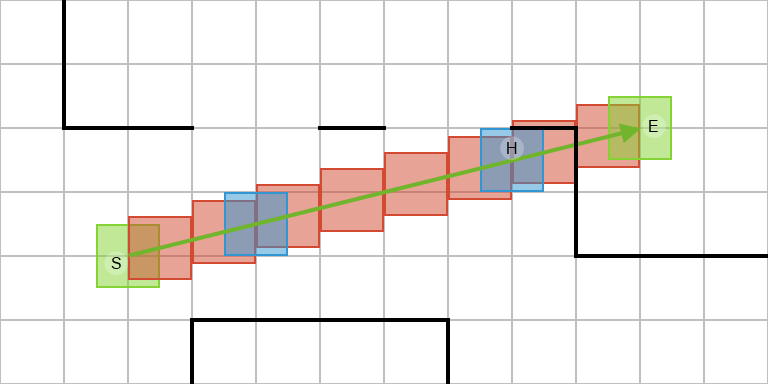
\includegraphics[width=0.9\textwidth]{trace}
\caption{A diagram to show the world geometry intersection checks performed when sweeping an object's bounding rectangle along a trace line. The object starts at position $S$ and its destination is position $E$. Black lines represent solid walls. The red boxes show iteration steps where a horizontal collision test is performed against possible obstructions to the right and the blue boxes are iteration steps where vertical collision tests are performed upwards. Position $H$ is the projected box location where a collision is first detected and so will be the position the object is moved to.}
\label{fig:trace}
\end{figure}

This technique compares well against the usual na\"{i}ve approach of sweeping a certain fixed distance along the movement vector each iteration. It is guaranteed to find an intersection if one exists and calculate the exact distance the object would have to travel to reach it rather than just the previous iteration location when using a constant step distance. It also requires fewer iterations, assuming a constant step distance approach uses a small iteration delta (which it would need to for accurate results).

\subsubsection{Subsumption Prototype}\noindent
Central to a subsumption agent architecture is a stack structure upon which behavioural layers can be pushed. This is relatively simple to implement using an Object Oriented approach and an adaptation of the design used by \citename{butler01} \citeyear{butler01} has been used involving an abstracted behavioural layer class with a method to be overridden that is called when that layer should decide to act. This method will return $true$ if it wishes to suppress the actions of lower layers, and otherwise $false$. The highest layer in the stack is invoked first and if that layer returned $false$ the next layer will be invoked. This continues until either a layer returns $true$, or the last layer has been invoked. The layers used in the final implementation are listed below, with the top-most layer first.

\noindent
\small{
\begin{itemize}
\layer{DropResource}{Drop a carried resource if in danger or at a barricade under construction}
\layer{SelfDefence}{Attack a pursuer if they are too close}
\layer{Mob}{If there are many more humans than zombies nearby, head towards a zombie}
\layer{VacateBlock}{If carrying a resource or in danger while inside a building, run outside}
\layer{Flee}{Run away from nearby danger}
\layer{PickupResource}{If standing on a resource and not in danger, pick it up}
\layer{FindResource}{If not in danger and not holding anything, move towards a resource}
\layer{HarvestResource}{Attack a nearby object that yields resources when broken}
\layer{SeekRefuge}{When outside and neighbouring a safe-looking building, run inside it}
\layer{Wander}{Walk around randomly}
\end{itemize}}

This particular configuration of behaviours were designed to satisfy each requirement of the AI prototype, using complimentary sets of layers to allow for more complex compound behaviours to emerge. The survival strategy is implemented with the $SelfDefence$, $Mob$, $VacateBlock$, $Flee$ and $SeekRefuge$ layers, and the remainder (along with $VacateBlock$ and $SeekRefuge$ again) are for constructing barricades autonomously.

The survival aspect functions with several emergent sub-strategies. The $SelfDefence$ behaviour will attack a zombie that is extremely close to the agent, which is expected to occur when the zombie catches up to the agent due to a movement speed advantage or if the agent has been chased into a corner. In either case, attacking the pursuer is the only rational thing left to do. The $Mob$ behaviour actively directs an agent towards a nearby zombie if that agent predicts that a decent number of other agents will perform the same action, enough to overwhelm the zombie. When the agents are close enough, the $SelfDefence$ behaviour will take control and cause the agents to attack the surrounded enemy. This strategy will lead to zombies being eliminated in safe situations where it is unlikely for a human agent to take much damage. $VacateBlock$ and $Flee$ will help avoid situations where being in close proximity to a zombie is unnecessary and $SeekRefuge$ ensures agents aren't exposed outside.

Barricade construction relies on a similar interaction between several behaviours. The process usually starts with an agent wandering around outside, carrying no resource object. The $SeekRefuge$ behaviour will lead it to navigate inside a building, within which it may find objects that yield resource items when damaged when obeying the $HarvestResource$ behaviour. When the object breaks into its component resources, the $PickupResource$ behaviour is followed and the agent now holds a resource item. The $VacateBlock$ layer instructs the agent to leave the building if it is holding a resource and as soon as the agent leaves it drops the item as instructed by the $DropResource$ layer. The agent then attempts to $SeekRefuge$ again and the cycle repeats. Resource items are continually dropped onto tiles neighbouring an exit to the building, which pile up to form barricades. When the barricade becomes large enough, the tile it belongs to becomes solid and the agent automatically finds a different path to leave and re-enter the building, thereby dropping items onto a different tile.

Each layer in this solution was quite trivial to implement due to their simplicity in isolation, although the overall organisation of layers involved a significant amount of planning. Some behaviours, such as $Mob$ and $Flee$, provided some scope for experimentation by testing different thresholds for when to perform that action, with values eventually chosen that balance survival rate against computational expense. Additionally, experiments were performed to test whether it was optimal for all agents to possess the $Mob$ layer, or if having a subset of agents that deviated from that strategy would lead to that set lasting markedly longer than the longest surviving agents in the first instance. This did not turn out to be the case, with the larger zombie population caused by having fewer courageous survivors leading to the overall survival rate decreasing.

\subsubsection{BDI Prototype}\noindent
For the BDI agent architecture an implementation for each of the three core components (Beliefs model, Desires identification and Intentions filtering) was developed as individual systems \cite{rao95}. After this, a set of desire types and their corresponding intentions was produced.

The Beliefs component involved designing a system for representing aspects of an agent's environment that could influence its actions, updating that internal representation as the agent perceives stimuli. The most direct structure for this model of the environment (while guaranteeing that potentially useful information is stored) would be to store every detail exactly as it is perceived; but this would be difficult to parse, would hold unnecessary detail and could result in too much memory being consumed. A better approach would be an abstracted model, and this implementation considers two levels of abstraction as with the path-finding solution (see section~\ref{sec:paths}). The highest level abstraction is at a city block scale, considering observed attributes of the contents of each block. Each agent tracks a few key properties about each block; the last time they observed it, whether that block contains a building, the number of human agents seen within that block, the number of zombie agents and the number of barricade resources seen. Each agent also tracks the locations of observed agents and resources for their local environment, information that is discarded when they travel a specified distance from the last place those entities were seen or after a long period of being unobserved to save memory. Agents also record whether they are within a building or outside, their health value and whether they are holding an item.

Desire identification is the next core component of the architecture, which involved designing a mechanism to parse the beliefs model to find a set of achievable goals that align with the higher aspirations of the agent. For this specific scenario, these aspirations revolve ensuring the agent's survival. This high level goal can be broken down into sub-goals as described by Figure~\ref{fig:goals}.

\label{sec:bdi}
\begin{figure}[h]
\centering
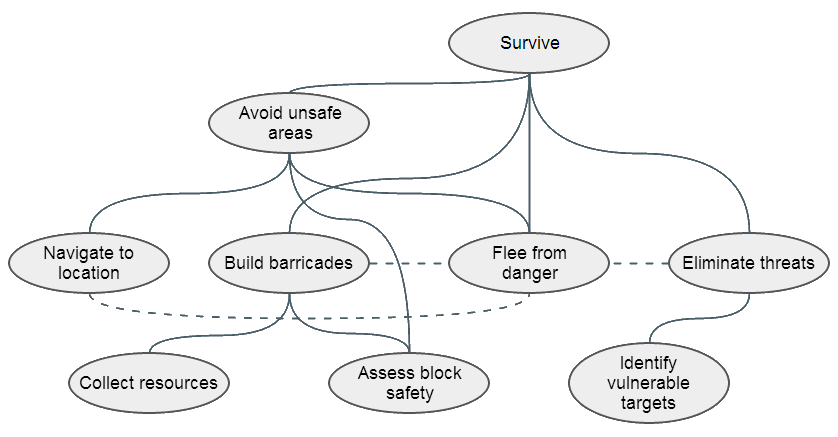
\includegraphics[width=0.8\textwidth]{goals}
\caption{A diagram to show a breakdown of the main goals for a human agent into sub-goals, with possible conflicts signified by dashed lines.}
\label{fig:goals}
\end{figure}

The \emph{Avoid unsafe areas} sub-goal obviously relies on being able to identify whether an area is potentially hazardous and more importantly whether there is another location worth travelling to due to increased expected safety. The implementation for this can exploits the abstracted block-level representation of the world as defined in the Beliefs model by calculating a \emph{utility} heuristic for each block. This heuristic is a function of the remembered number of zombies, humans, barricade resources and taking into account uncertainty related to the amount of time since the block was last observed. While a functional heuristic has been developed, further experimentation may be performed to maximise its quality. A second heuristic is then be calculated for each block which finds the estimated cost of travelling there. If any blocks are deemed to be safer than the one the agent currently resides in (using the first heuristic) and is also found to be worth the trip (using the second heuristic), the agent will desire to travel to it.

For the \emph{Eliminate threats} sub-goal, agents need to rely on teamwork to safely and efficiently attack zombies. A one-on-one fight will lead to the human receiving a considerable amount of damage, whereas if a large group of humans attack an individual target the fight will be resolved quickly before much damage is dealt by the zombie. For this cooperative strategy to work, agents need to determine if enough other agents will be willing to pitch in for the battle to be worth undertaking. This has been achieved by each agent independently being empathetic towards other agents within a certain range of the prospective target, testing to see if each of them are expected to join in on the fight. If it is estimated that a sufficient number would cooperate, a desire to attack the target is included with the desire set. As a fail-safe for when guessing the intentions of other agents fails, if an agent finds itself considerably closer to a zombie than other agents it will forfeit the desire to attack it in favour of desiring to flee.

Barricade construction desires are produced if an agent is within a block with a large number of other survivors and a sufficient number of resources, with the absence of zombies or an existing barricade. This desire obviously conflicts with any desires to migrate to other blocks, and so is filtered out if any such desires are present. If a barricade construction desire survives the filtering process, its corresponding intention plans which specific tiles require barricading within the target block upon creation. It then efficiently navigates the agent between barricade resources and where they should be placed until the barricade is complete, at which time the intention recognises this to be the case and removes itself.

There are two possible points of contention that may arise during the BDI architecture's main loop; conflicting desires and conflicting actions. A single solution to both issues has been produced by providing an interface used by both desire types and action types, where each pair in the desire or action set is tested for a conflict and the element with the highest utility heuristic decides how the conflict is resolved. For example, movement actions are resolved by combining their respective vectors, weighting each by its attached utility, then normalising the result to ensure the agent doesn't move slowly. The same applies for desires to avoid two different threats; a combined desire is produced to move in a direction that moves away from both threats simultaneously if possible, with a weighting dependant on how close each threat is.

The beliefs update process is staggered to occur every few simulation steps per agent, and the desire deliberation process occurs even less frequently unless an intention declares that it should be removed. This is to improve the average simulation time for each agent, which ensures the simulation can be performed fast enough to maintain an adequate frame update rate. While more frequent beliefs updates mean an agent can respond to changes in its environment faster, it is expected for intentions to be committed to for significant periods of time \cite{bonura09} so the reduced deliberation rate for changing intentions does not affect the rationality of each agent much.

\subsubsection{Analysis Strategy}\noindent
A comprehensive and fair analytical method is required for comparing the two agent architectures and this section will cover a set of experiments that satisfy both of these qualities.

\textbf{Survival Rate} will be tested by first selecting a set of initial simulation states (at least 10) and running the simulation using each once per agent architecture. Each simulation will be left to run for 5 minutes and the number of survivors and zombies at each moment in time will be logged. The data produced will be used to produce graphs of the agent counts over time which can be analysed in terms of population decline rates, time until a stable population is established and whichever other statistical features that may appear. This test will involve no player interaction, only the purely autonomous aspects of the agent designs.

\textbf{Task Completion} will analyse the efficiency at which each agent design can complete tasks assigned by a player. Similarly to the survival rate test, a set of initial states will be produced over which both architectures will run, the difference being that each initial state will include an instruction to build a collection of barricades at specific locations. The simulation will execute until each barricade is completed, the progress towards completion being recorded over time. This data will be graphed and compared, as with the survival rate data.

\textbf{Performance} of the two architectures is of obvious importance; a solution with optimal survival rate and task completion efficiency has little use if it can only support a handful of agents at a time without reducing the simulation to an agonisingly slow crawl. The main method for the survival rate test can be used here, but with frame-time (the time taken to calculate each simulation step) being recorded rather than survival rate. The main requirement for the architectures is to keep average frame-time below 16.67ms, with minimal dips above that threshold. This test is platform dependant and so will be carried out on at least two different machines. Additional more superficial tests will also be performed with world sizes spanning from 64x64 tiles to 256x256 tiles and a range of agent counts from 50 to 1000 with each world size, to analyse performance relating to dense vs sparse populations.

\newpage
\section{Results}
\noindent
Quantitative results were produced by running the subsumptive architecture and two versions of the BDI implementation (one with frequent belief and deliberation updates, and the other with one quarter of the frequency) on a total of 160 different initial world states. These were divided into 8 different categories of world size and initial agent populations, designed to test different population densities, total agent counts, and ratios of survivor agents to antagonistic ones. For each of these categories 20 seeds were used to control the specific geometry generated and placement of agents, giving the total of 160 distinct environments. Table \ref{tab:environs} lists each of the categories used to produce the final set of results.

\begin{table}[ht]
\centering
\begin{tabular}{|c|c|rcl|c|c|} \hline
{\bf ID} & {\bf Size} & {\bf Agents} & : & {\bf Threats} & {\bf Agent Ratio} & {\bf Agent Density} \\ \hline
A & 64 & 48 & : & 16 & 3 : 1 & 1.172 \\
B & 64 & 96 & : & 32 & 3 : 1 & 2.344 \\
C & 64 & 120 & : & 8 & 15 : 1 & 2.930 \\ \hline
D & 128 & 96 & : & 32 & 3 : 1 & 0.586 \\
E & 128 & 120 & : & 8 & 15 : 1 & 0.732 \\
F & 128 & 128 & : & 128 & 1 : 1 & 0.781 \\
G & 128 & 192 & : & 64 & 3 : 1 & 1.172 \\
H & 128 & 224 & : & 32 & 7 : 1 & 1.367 \\ \hline
\end{tabular}
\caption{The 8 different initial environment categories, for each of which 20 distinct instances were used for testing. Agent density measures the mean number of survivor agents per 100 tiles.}
\label{tab:environs}
\end{table}

Each of the 480 individual tests ran for 36,000 individual simulation ticks, which is equivalent to 10 minutes of simulation time at 60 ticks per second. Every time the agent population changed a datapoint would be logged; recording the current time, the number of agents of both types, and the average time spent per tick to simulate the agent AI. The data for each of the 20 instances in a category was then aggregated into a single graph of averaged data, with plots for each AI implementation for comparison. This provided a set of 16 graphs in total, six of which are on the following pages to illustrate points identified during their evaluation. Additionally, Table \ref{tab:results} lists the mean final population counts for the three algorithms tested, along with their mean frame time per agent.

\begin{table}[ht]
\centering
\begin{tabular}{|c|c|c|c|c|c|c|} \hline
& \multicolumn{3}{c|}{\bf Average Agent Count} & \multicolumn{3}{c|}{\bf Average Frame Time (ms)} \\ \hline
{\bf \small ID} & {\bf \small Slow BDI} & {\bf \small Fast BDI} & {\bf \small Subsump} & {\bf \small Slow BDI} & {\bf \small Fast BDI} & {\bf \small Subsump} \\ \hline
A & 29.2 & 23.3 & 24.6 & 0.777 & 0.365 & 0.692 \\
B & 52.4 & 38.0 & 44.7 & 1.343 & 0.741 & 2.057 \\
C & 116.0 & 114.4 & 114.0 & 2.209 & 1.230 & 5.288 \\ \hline
D & 69.8 & 61.6 & 58.9 & 1.678 & 0.971 & 1.893 \\
E & 114.7 & 111.7 & 110.8 & 2.333 & 1.381 & 4.390 \\
F & 30.6 & 23.9 & 19.7 & 1.054 & 0.714 & 0.757 \\
G & 125.4 & 98.7 & 96.9 & 2.954 & 1.990 & 3.099 \\
H & 195.9 & 176.1 & 182.8 & 4.206 & 2.265 & 6.364 \\ \hline
\end{tabular}
\caption{Final agent counts and frame times for each algorithm on each initial state category (as specified in Table \ref{tab:environs}).}
\label{tab:results}
\vspace{-20mm}
\end{table}

\begin{figure}
\vspace{-20mm}
\centering
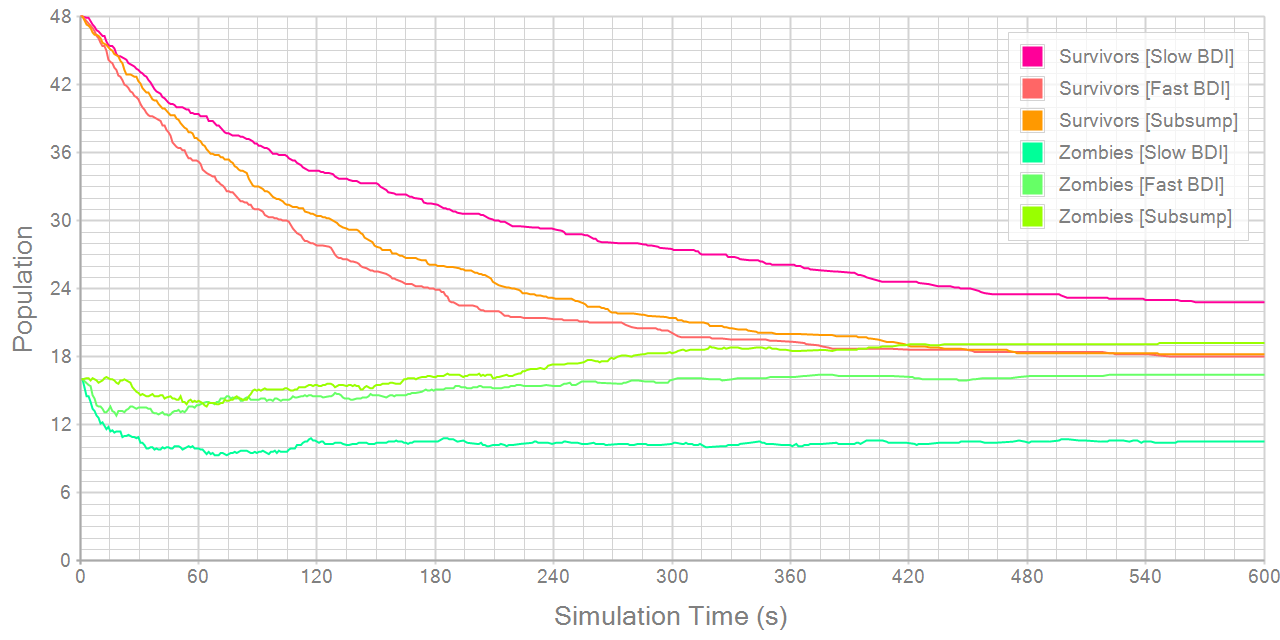
\includegraphics[width=0.8\textwidth]{../../Results/64_48_16/population}
\caption{\small Average population curves for the 60 simulations on a world of size 64x64, with an initial 48 survivors and 16 zombies.}
\label{fig:64_48_16_pop}

\vspace{5mm}
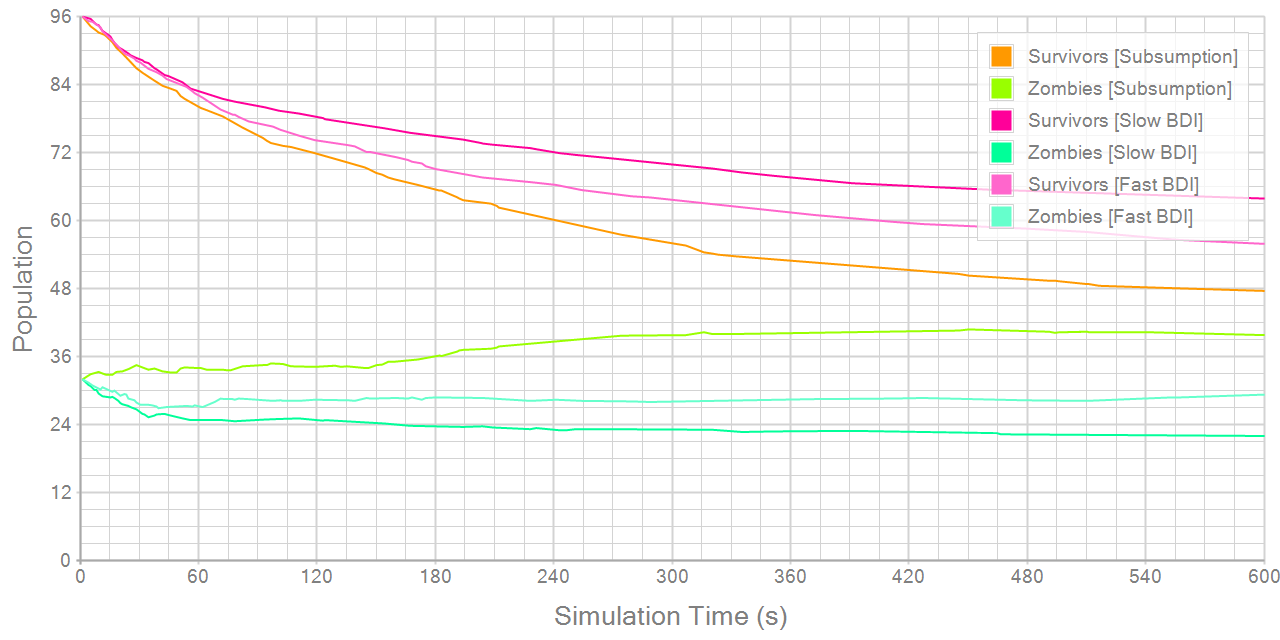
\includegraphics[width=0.8\textwidth]{../../Results/128_96_32/population}
\caption{\small Average population curves for the 60 simulations on a world of size 128x128, with an initial 96 survivors and 32 zombies.}
\label{fig:64_96_32_pop}

\vspace{5mm}
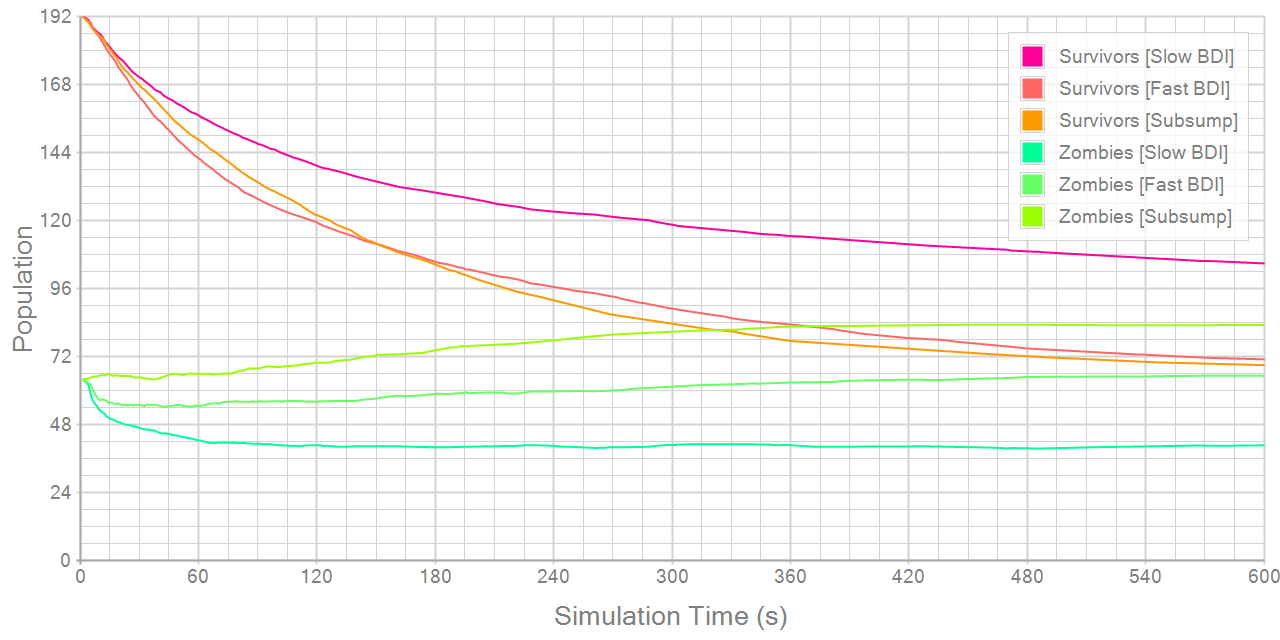
\includegraphics[width=0.8\textwidth]{../../Results/128_192_64/population}
\caption{\small Average population curves for the 60 simulations on a world of size 128x128, with an initial 192 survivors and 64 zombies.}
\label{fig:128_192_64_pop}
\end{figure}

\begin{figure}
\vspace{-20mm}
\centering
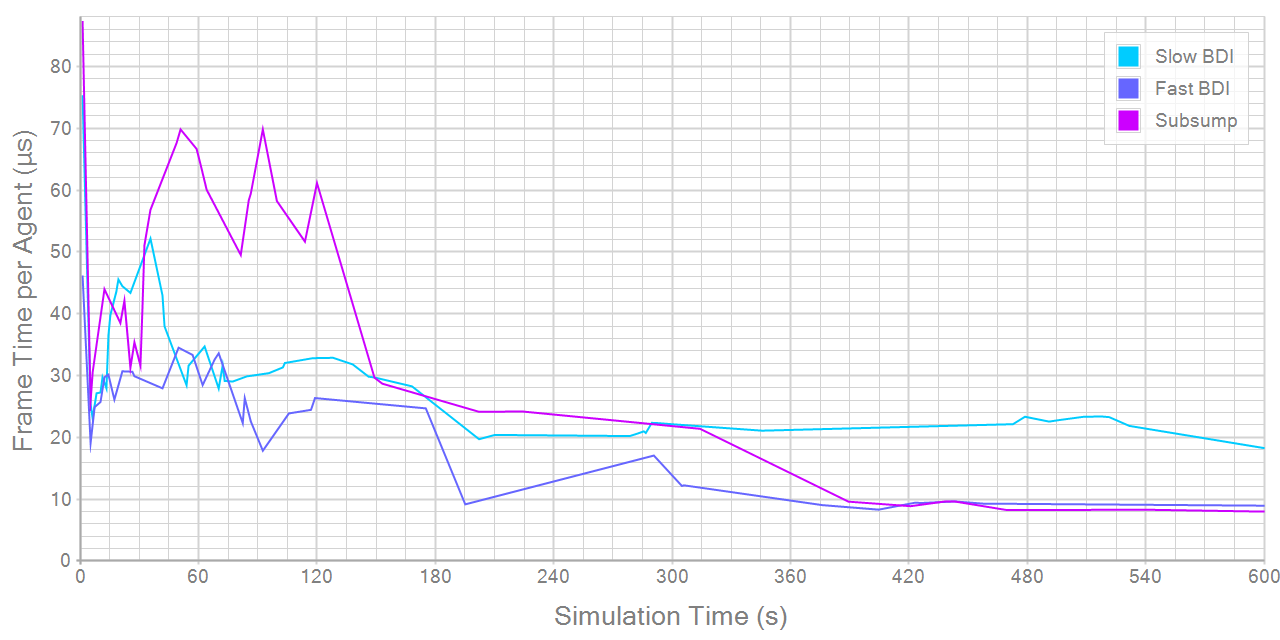
\includegraphics[width=0.8\textwidth]{../../Results/64_48_16/performance}
\caption{\small Average AI simulation performance for the 60 simulations on a world of size 64x64, with an initial 48 survivors and 16 zombies.}
\label{fig:64_48_16_per}

\vspace{5mm}
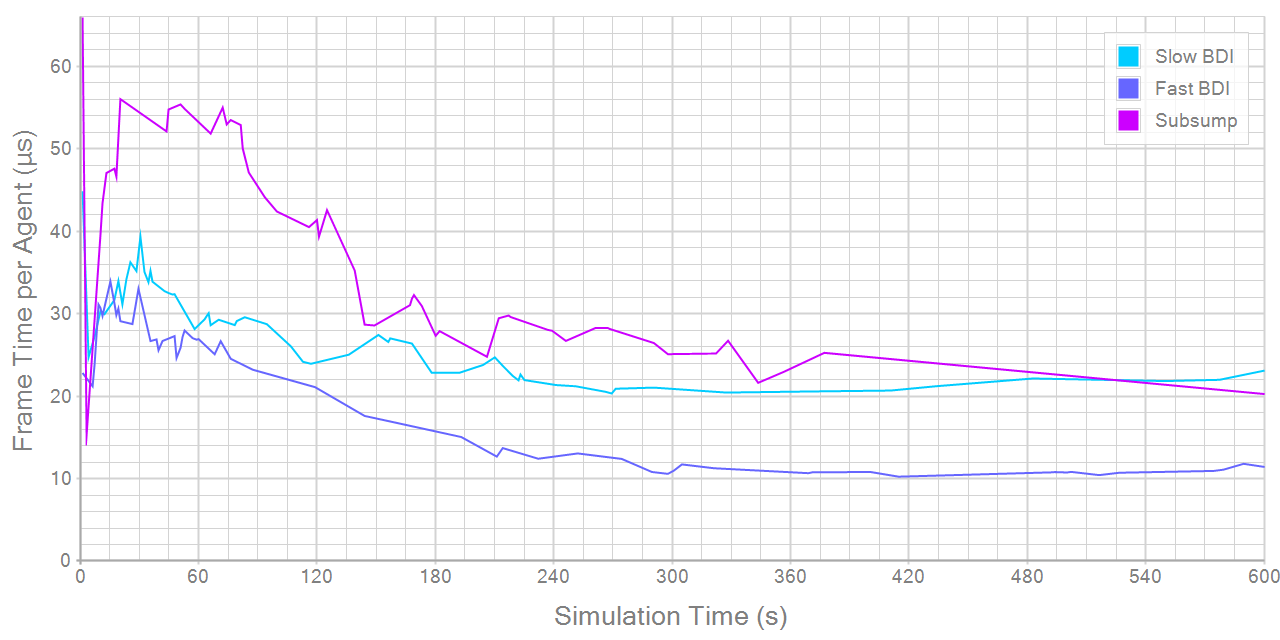
\includegraphics[width=0.8\textwidth]{../../Results/128_96_32/performance}
\caption{\small Average AI simulation performance for the 60 simulations on a world of size 128x128, with an initial 96 survivors and 32 zombies.}
\label{fig:64_96_32_per}

\vspace{5mm}
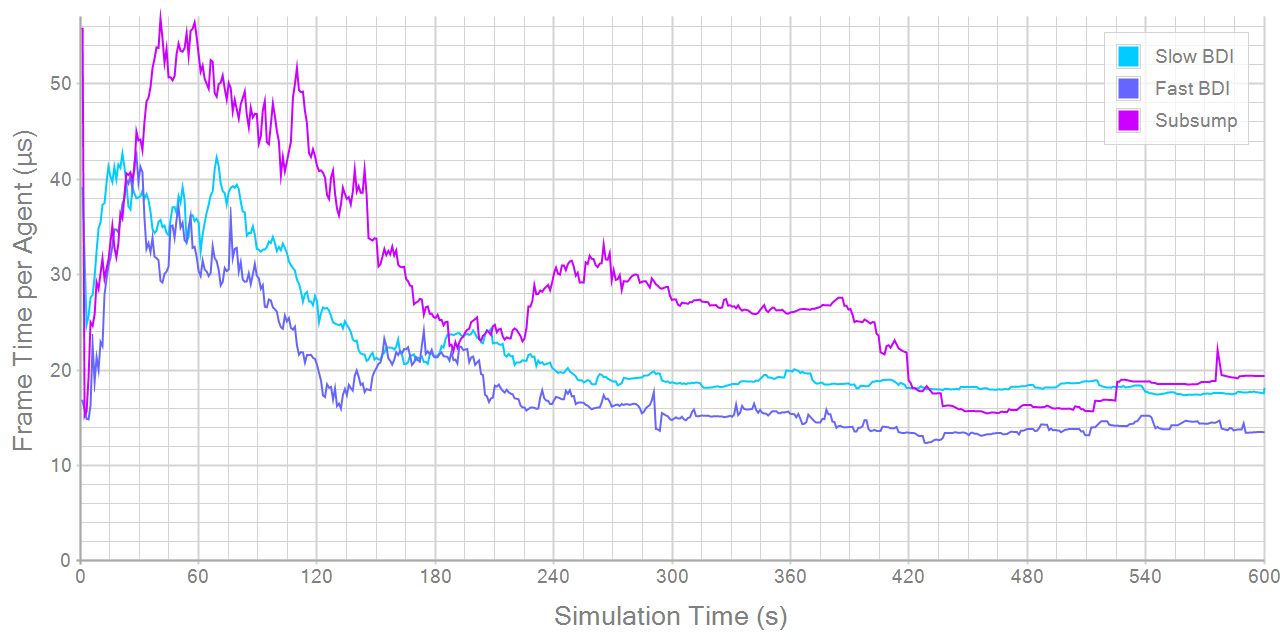
\includegraphics[width=0.8\textwidth]{../../Results/128_192_64/performance}
\caption{\small Average AI simulation performance for the 60 simulations on a world of size 128x128, with an 192 survivors and 64 zombies.}
\label{fig:128_192_64_per}
\end{figure}

\section{Evaluation}
\noindent
The survival rate plots clearly demonstrate that one implementation is the most successful at maintaining the agent population, with the more intensive BDI implementation outperforming the others significantly in all instances. The subsumption and less intensive BDI implementations appear to be very similar in terms of survival rate, with the fast BDI maintaining a slightly higher mean population count overall.

As the two BDI implementations differ only in the frequency that the individual agents update their belief databases and deliberate on new intentions, so the considerable difference in survival rates demonstrates that those higher frequencies are certainly advantageous. This will be because a higher belief and intention update frequency allows the agents to respond to a dynamic environment with a lower mean latency, or in other words they have faster reflexes.

Each of the behaviours in the subsumption architecture are polling their respective agent's environment with an equivalent or higher frequency compared to the high-frequency BDI implementation, so a difference in response latency is not the source of the disparity in survival rates between the two algorithms. However, when watching the two algorithms execute an obvious issue with the subsumption architecture becomes apparent that will be a large factor in reducing agent survival rates. There are clear instances where two behaviours will ``fight'' each other for control of the agent; for example a behaviour to leave a building will cause an agent to step outside, only for a subsumed behaviour to send the agent back inside during the next simulation step. This will continue until another behaviour breaks up the fight, like the fleeing behaviour causing the agent to run further inside. This will lead to neither behaviour achieving their respective goals, and would require either far more complex and therefore expensive logic in each behaviour or communication between behaviours which would violate one of the core principles of the architecture. The BDI implementations avoid such conflicts of interest by aggregating the actions requested by each current intention, placing precedence on whichever has the highest attached utility heuristic. Movement actions are normalised after aggregation, so an agent won't experience restricted movement if it has two intentions pulling it in opposite directions but will instead move at full speed in whichever direction has the highest utility. This is far more rational behaviour, and subjectively appears more natural than the occasionally indecisive subsumption approach.

While the population decline plots show relatively similar behaviour between the different approaches, the frame time data tells a vastly different story. The first thing to note is the large range of frame rates for the subsumption architecture in each graph, suggesting the frame time is wildly unpredictable and so unsuitable for a real-time game environment. The larger peaks near the start of each graph (which the BDI plots also exhibit, albeit in a far more muted form) will be caused by the relatively high density of agents near the start of the simulation, meaning each agent must consider a larger number of nearby objects. The subsumption architecture will suffer more from this as each behavioural layer individually examines its local environment without the processing being shared between them. In comparison, the BDI approach only samples its environment during beliefs updates, the results of which are shared between all desire and intention types that may require them.

Some more trivial observations include the apparent significant benefit in reducing belief and deliberation update frequency for the BDI approach in terms of running time, although admittedly at the cost of agent survival rate. This very simple modification to vary the algorithms efficiency would be very useful in a game setting, where a player may wish to adjust the AI's quality to a level that performs well on their device. The subsumptive architecture cannot be adjusted in such a simple way, and would require each behavioural layer to accommodate a variable quality level independently. Another observation is that running time per agent for the BDI approaches settles down to a near constant value after the initial peak of high population density. Such a steady and predictable processing time would equate to a steady display update rate, meaning a player won't be subjected to intermittent periods of low frame rates that may disrupt their experience.

From a programmer's perspective, the subsumptive architecture itself was relatively trivial to implement, and each individual behavioural layer is extremely simple as they each are only concerned with one sub-problem of an agent's overall agenda. However, the main difficulty lies in deciding which layers to add and in what order, as complex interactions between individual behaviours are relied on for complex compound behaviours to emerge. Additionally, while certain constructive interactions between the layers may be anticipated and utilised, unexpected destructive interactions may arise such as two competing layers leading to an indecisive agent.

Conversely the implementation of the BDI architecture was much more involved; with quite a bit of effort involved in designing the beliefs database, the desire capturing, filtering and ordering process, intention deliberation, and action aggregation. Thankfully the process of designing and implementing each desire and intention type was far simpler after the underlying architecture was in place, with fewer concerns about how the desires could potentially interact and instead relying on an automatic conflict resolution system between desires and actions. This system has the additional benefit of being easily extensible, whereas the process of adding additional behaviours to the subsumption model would require careful consideration about how potential new layers would interact with existing ones.

Overall, this implementation of the BDI architecture seems to fit this particular scenario well, meeting each of the core requirements of increasing survival rate, performing complex tasks like barricade construction, being computationally inexpensive, and navigating the environment rationally while avoiding unnatural looking behaviour. The subsumption architecture was not as successful in all of these aspects, and additionally was more difficult to implement due to the reliance on complex interactions between behavioural layers.

\section{Conclusions}
\noindent
Performing this analysis of the comparative merits and shortcomings of the subsumption architecture and BDI model for this particular problem instance has certainly been worthwhile, as the results deviate from what may be expected in several respects.

Due to its bulky underlying architecture it may be assumed that the BDI approach would suffer from poorer performance, but it is now evident that this bulk offsets calculations that would otherwise be performed by each individual behavioural layer in a subsumption-based implementation. It is additionally trivial to tweak the performance of the BDI implementation (at the cost of quality), allowing for the possibility of users on less capable machines experiencing an acceptable simulation speed. The BDI implementation also maintained a far more stable execution time for each agent, which translates to a smoother gameplay experience.

It may also be assumed that the subsumption approach would be the easiest to implement, but that turns out to only be true for the underlying architecture. The internals of a decently implemented BDI framework offsets a significant portion of the programming that would otherwise be involved in the implementation of each atomic behaviour, leading to both simpler code and a more efficient solution.

Under subjective analysis the BDI implementation is again more successful for this problem domain, granting the actions of the agents a more natural appearance rather than the occasionally indecisive anomalous behaviour of the agents being controlled by a subsumption stack.

It is therefore fair to conclude that the BDI model implementation for this project is a better fit for the original problem scenario than the subsumption-based approach, and so will be used as the basis for the AI during the continued development of this game project.

There are a few possible avenues for extension of the BDI implementation that may be of value. One is the implementation of shared plans for tasks like barricade construction or the exploration of territory, where one agent coordinates a group of subservient workers. This allows for more coordinated actions while also reducing the time spent deliberating on plans by offsetting the planning of many agents to just one. A further extension would be a more complex barricade design system; currently barricades are only constructed across the entrances of buildings, but this can be improved by having agents decide to block off entire streets of the city to enclose a larger area. This would fit well with the proposed plan sharing system, and would lead to more interesting and possibly more successful agents.

\bibliography{projectpaper}

\end{document}